\documentclass[a4paper]{exam}

\usepackage{geometry}
\usepackage{graphicx}
\usepackage{hyperref}
\usepackage{titling}

\printanswers

\title{Weekly Challenge 01: Comparison\\CS/MATH 113 Discrete Mathematics}
\author{Ali Muhammad Asad - TA}  % <== for grading, replace with your team name, e.g. q1-team-420
\date{Habib University | Spring 2023}

\qformat{{\large\bf \thequestion. \thequestiontitle}\hfill}
\boxedpoints

\begin{document}
\maketitle

\begin{questions}
  
\titledquestion{Safety at the Carnival}
  \begin{minipage}{.3\linewidth}
  \centerline{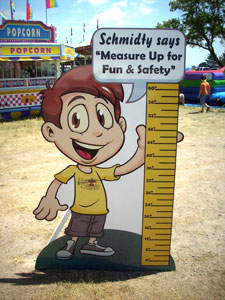
\includegraphics[width=\textwidth]{height}}
\end{minipage}
  \begin{minipage}{.65\linewidth}
Schmidty \cite{schmidt} has grown old and his vision is weak. He can no longer see if a person meets the height limit. The carnival organizers have installed a sensor to help. It beeps if any of the people in the waiting area is not eligible. Schmidty can move people in and out of the waiting area and then apply the sensor.

  \begin{parts}
  \part A family of 5 is trying to sneak in their toddler who does not meet the limit. Describe how Schmidty can identify the toddler in no more than 3 applications of the sensor.
  \part What is the smallest number of times that Schmidty needs to apply the sensor for a family of size $n$ in which only one person is below the limit. Justify your answer.
  \end{parts}
\end{minipage}
\begin{solution}
    % Enter your solution here.
    (a) Schmidty can first divide the family into two groups of 3 and 2 respectively, it doesn't matter how he does it, only that he divides the family of 5 into two groups of 3 and 2. \\ 
    He uses his sensor first at the group of 3. If it does not beep, then he can infer that the group of 2 will have the person with height less than the limit. So he can again divide the group of 2 into individuals, and apply the sensor a second time on either of the person. If it the sensor beeps, then we have found our person. If the sensor does not beep at the person, then the sensor can be applied a third time on the last person, in which case it will beep. \\ 
    If the sensor does beep at the group of 3 people in the first application, then he can again divide the group of 3 into a group of 2 and 1 (again the order does not matter). He applied the sensor then a second time at the group of 2; if it does not beep, then the last person will be the one with height less than the limit and a third application of the sensor will verify. If the sensor does beep on the second application at the group of 2, then the person is in either of the two people. The group can then again be divided into individuals, and then the sensor can be applied a third time to either of the individuals. If the sensor beeps, then we have found our person, if the sensor does not beep, then the last person is the person with height less than the limit.
    
    (b) For a family of size $n$, the family can be divided into two such that there are two groups of size $ \frac{n}{2} $ and then the sensor can be applied to either of the group. If it beeps then the person is in that group, else the person is in the other group. Then the group of $ \frac{n}{2} $ will again be divided into two such that there are two groups of $ \frac{n}{4} $ and again the sensor will be applied to either of the two groups. If the sensor beeps, then the person belongs to that group, else the person belongs to the other group. The process can be repeated until we are left with two individuals, and the sensor can then be used on either of the two. Then the least number of times the sensor has to be used turns out to be $ \log_{2}n + 1$.
  \end{solution}
\end{questions}

\begin{thebibliography}{9}
\bibitem{schmidt}
  TJ Schmidt \& Company (Standish, MI). \emph{Safety \& Maintenance}. \url{https://tjschmidtcarnival.com/pageserver/safety}. \textit{Last accessed on 6 Jan, 2023}.
\end{thebibliography}

\end{document}

%%% Local Variables:
%%% mode: latex
%%% TeX-master: t
%%% End: